\chapter{Programování testeru}

\label{sec:config}
\section{Konfigurace testeru}
Veškerý software testeru je k dispozici ve zdrojovém kódu.
Překlad modulů je řízen pomocí \lname{Makefile}. Vývoj byl proveden
na Ubuntu Linux s nástroji GNU (GNU toolchain, gcc verze 4.5.3).

Je jistě lehce možné, používat jiné operační verse Linuxu.
Načtení přeložených dat do paměti flash nebo do paměti EEPROM
je provedeno programem '\lcmd{avrdude}' \cite{avrdude} (Version 5.11svn) při použití \lname{Makefile} volbou \lcmd{make upload}.\\
 Program '\lcmd{avrdude}' je k dispozici pro Linux a Windows.
Kompilátor GNU C je také používán softwarem AVR studio v systému Windows pomocí softwaru WinAVR \cite{winavr1},\cite{winavr2}.

Můžete také načíst programová data (.hex a .eep) s jinými programy do ATmega,
ale pouze moje \lname{Makefile}  verze zajišťuje, že se dostanou správná data do zvoleného procesoru.

'\lcmd{avrdude}' načítá data do ATmega pouze tehdy, pokud jsou bajty podpisu připojené ATmegy stejné jako vybrané.
Pokud změníte \lname{Makefile}, bude software kompletně přeložen, pokud zvolíte \lcmd{make} nebo
\lcmd{make upload}.

Software, který byl přeložen pro ATmega8, nefunguje na ATmega168 a
software, který byl přeložen pro ATmega328, nefunguje na ATmega168.

Výjimkou je software, který byl přeložen pro ATmega168. Tyto soubory programu
jsou také užitečné pro ATmega328.
Dávejte pozor, při použití jiné, než s testerem dodané \lname{Makefile}.
S příslušnými možnostmi je software také založen na nezměněném návrhu hardwaru
Markus F. spustitelný (PARTNO=m8 , {\textbf ne} NO\_AREF\_CAP a {\textbf ne} možnost PULLUP\_DISABLE).
Taktová frekvence může být také nastavena pojistkami (fuses) na \(8MHz\), pak není nutný krystal!

K konfiguraci softwaru pro tester jsou k dispozici následující volby v \lname{Makefile}:

\begin{description} \setlength{\itemsep}{0em}
  \item[PARTNO] popisuje cílový Procesor:\\
         m8 = ATmega8\\
         m168 or m168p = ATmega168\\
         m328 or m328p = ATmega328\\
         m644 or m644p = ATmega644\\
         m1284p        = ATmega1284\\
         m1280         = ATmega1280\\
         m2560         = ATmega2560\\
    Příklad: PARTNO = m168
  \item[UI\_LANGUAGE] volba možné řeči pro tester:\\
    LANG\_BRASIL, LANG\_CZECH, LANG\_DANISH, LANG\_DUTCH, LANG\_ENGLISH, \\
    LANG\_GERMAN, LANG\_HUNGARIAN, LANG\_ITALIAN, LANG\_LITHUANIAN, \\
    LANG\_POLISH, LANG\_RUSSIAN, LANG\_SLOVAK, LANG\_SLOVENE, \\
    LANG\_SPANISH, und LANG\_UKRAINIAN lze nyní použít.
 Ruské a ukrajinské jazyky vyžadují LCD s cyrilikou.\\
    Příklad: UI\_LANGUAGE = LANG\_ENGLISH
  \item[LCD\_CYRILLIC] je potřeba pouze při použití displeje s cyrilickým charakterem.
Znaky \(\mu\) a \(\Omega\) nejsou zahrnuty v cyrilické znakové sadě.
Pokud tuto možnost určíte, oba znaky budou načteny do LCD softwaru.
Tuto volbu nastavíte, pokud se ve výstupu namísto \(\mu\) nebo \(\Omega\) objeví nesprávné znaky.\\
Příklad: CFLAGS += -DLCD\_CYRILLIC
  \item[LCD\_DOGM] musí být zadán, když používáte displej s ovladačem ST7036 (typ DOG-M).
Kontrast LCD se pak nastavuje pomocí softwarových příkazů.
Pokud jste nastavili příliš velký kontrast, displej nezobrazuje nic,
Nejdříve se mohou pokusit zjistit, jestli je při pohledu na obrazovku ze strany něco vidět.
jinak by měl být EEprom přepisován, aby se změnila hodnota kontrastu.\\
Příklad: CFLAGS += -DLCD\_DOGM
  \item[FOUR\_LINE\_LCD] lze použít na displeji 4x20 znaků pro lepší využití místa na displeji.
Další parametry, které se jinak zobrazují pouze krátce na 2 řádku, jsou zobrazeny v na řádcích 3 a 4.\\
Příklad: CFLAGS += -DFOUR\_LINE\_LCD

  \item[DD\_RAM\_OFFSET] U některých textových zobrazení se rozlišují počáteční adresy DD-RAM pro začátek řádku. Normálně začíná první řádek na adrese DD-RAM 0.
U některých zobrazení jako TC1604 nebo TC1602 začíná 1 řádek, ale na adrese 128 (0x80).
Tuto možnost lze zvážit.\\
Příklad: CFLAGS += -DDD\_RAM\_OFFSET = 128

  \item[WITH\_LCD\_ST7565] Tato volba musí být použita při použití sériového LCD displeje o velikosti 128x64 pixelů.
Pro tento typ zobrazení je třeba nastavit další volby, které lze nalézt v tabulcee~\ref{tab:cod-display}.
Namísto ovladače ST7565 lze například nakonfigurovat podobný řadič SSD1306.
V tom případě musí být volba nastavena na 1306.
Ovladač PCF8812 nebo PCF8814 je také podporován, pokud je tato možnost nastavena správně.
Může být také připojen displej s řídicím systémem ST7920 nebo NT7108.
Pro regulátor NT7108 musí být použít další sériový měnič 74HC (T) 164 nebo 74HC (T) 595.\\
Příklad: WITH\_LCD\_ST7565 = 1 

 \item[LCD\_INTERFACE\_MODE] U řídicí jednotky SSD1306 je možné nahradit standardní 
SPI rozhraní (4-Wire) za rozhraní I\textsuperscript{2}C.
Tato volba musí být nastavena na hodnotu 2.
U ovladače regulátoru ST7920 lze nastavit speciální sériový port s touto volbou nastavenou
na hodnotu 5 je podporován.
Je-li k dispozici pouze jedna možnost připojení, nemusí být nastaven konstantní LCD\_INTERFACE\_MODE 
Všechny doposud možné hodnoty pro LCD \\ WITH\_LCD\_ST7565 a\\ LCD\_INTERFACE\_MODE jsou
uvedeny v tabulce~\ref{tab:cod-display}.

\begin{table}[H]
  \begin{center}
    \begin{tabular}{| c | c | c | c|}
    \hline
 Display-Typ        &  Interface     & WITH\_LCD\_ST7565 &  LCD\_INTERFACE\_MODE \\
    \hline
    \hline
  Character 16x2,   & 4-Bit parallel &  disabled (0)      & disabled (1) \\
  Character 20x4    & 4-Wire SPI     &                    &    4   \\
                  & I\textsuperscript{2}C &               &    2   \\
    \hline
  Graphic ST7565    & 4-Wire SPI      & 1 or 7565          & disabled (4) \\
    \hline
  Graphic ST7565  & I\textsuperscript{2}C & 1 or 7565     &   2 \\
    \hline
  Graphic SSD1306   & 4-Wire SPI      & 1306               & disabled (4) \\
    \hline
  Graphic SSD1306 & I\textsuperscript{2}C & 1306          &   2 \\
    \hline
  Graphic ST7920    & 4-Bit parallel  & 7920              & disabled (1) \\
    \hline
  Graphic ST7920    & 2-Bit serial    & 7920               &  5 \\
    \hline
  Graphic NT7108    & 8-Bit parallel  & 7108              & disabled (6) \\
  oder KS0108       &    + 74HCT164   &                   &      \\
    \hline
  Graphic PCF8812   & 4-Wire SPI      & 8812              & disabled (4) \\
    \hline
  Graphic PCF8814   & 4-Wire SPI      & 8814              & disabled (4) \\
                  & I\textsuperscript{2}C & 8814          &   2 \\
                    & 3-line          & 8814              &   3 \\
    \hline
  Graphic ILI9163   & 4-Wire SPI      & 9163              & disabled (4) \\
  128x128 Color     &                 &                   &              \\
    \hline
  Graphic ST7735    & 4-Wire SPI      & 7735              & disabled (4) \\
  128x160 Color     &                 &                   &              \\
    \hline
    \end{tabular}
  \end{center}
  \caption{Klíčové údaje pro typ řadiče a rozhraní}
  \label{tab:cod-display}
\end{table}

Hodnoty v závorkách jsou interně používány pouze softwarem a jsou zde uvedeny pouze pro informaci.
Hodnoty v závorce byste neměli zadávat v \lname{Makefile}.\\
Příklad: CFLAGS += -DLCD\_INTERFACE\_MODE=2
\item[LCD\_SPI\_OPEN\_COL] Pomocí volby LCD\_SPI\_OPEN\_COL se datové signály SPI rozhraní nepřepínají na VCC.
	Signály se přepínají pouze na GND, pro \inquotes{high} signály se přepínají na \inquotes{Pull-Up} odpory od ATmega.
Pro \inquotes{Reset} signál je však vyžadován externí odpor, pokud je volba PULLUP\_DISABLE nastavena.
Pro ostatní signály SPI jsou dočasně použity interní \inquotes{Pull-Up} odpory v mcu,
pokud je nastavena volba PULLUP\_DISABLE.\\
Příklad: CFLAG += -DLCD\_SPI\_OPEN\_COL
\item[LCD\_I2C\_ADDR] Die I\textsuperscript{2}C-adresa ovladače SSD1306 lze nastavit přednastavením adresy
LCD\_I2C\_ADDR na předem zvolenou adresu nastavit.\\
Příklad: CFLAGS += -DLCD\_I2C\_ADDR=0x3d
\item[LCD\_ST7565\_RESISTOR\_RATIO] Tato volba nastaví poměr děliče odporu pro
Regulátor napětí regulátoru ST7565. Užitečné hodnoty jsou obecně mezi 4 a 7.
Můžete nastavit hodnoty mezi 0 a 7. \\
Příklad: LCD\_ST7564\_RESISTOR\_RATIO = 4
\item[LCD\_ST7565\_H\_FLIP] Tato volba umožňuje otočit displej vodorovně.\\
Příklad: CFLAGS += LCD\_ST7565\_H\_FLIP = 1
\item[LCD\_ST7565\_H\_OFFSET] Tato volba může přizpůsobit paměť použitou pro výstupné okno displeje.
Řídicí jednotka používá více horizontálních pixelů (132) než je zobrazeno (128).
V závislosti na použitém zobrazovacím modulu může být pro správné zobrazení nutné použít hodnotu 0, 2 nebo 4.\\
Příklad: CFLAGS += LCD\_ST7565\_H\_OFFSET = 4
\item[LCD\_ST7565\_V\_FLIP] Tato volba umožňuje otočit displej svisle.\\
Příklad: CFLAGS += LCD\_ST7565\_V\_FLIP = 1
\item[VOLUME\_VALUE] Zde můžete nastavit hodnotu kontrastu pro ovladač ST7565 nebo SSD1306.
Hodnota může být pro regulátor ST7565 mezi 0 a 63.
Pro regulátor SSD1306 jsou povoleny hodnoty mezi 0 a 255 \\
Příklad: CFLAGS += -DVOLUME\_VALUE = 25
\item[LCD\_ST7565\_Y\_START] Pomocí této volby může být první řádek nastaven svisle správně.
Pro některé varianty zobrazení je první řádek posunut do středu obrazu.
Tyto displeje přesouvají první řádek zpět nahoru
pokud je tato možnost nastavena na hodnotu 32 (výška poloviny obrazovky).\\
Příklad: CFLAGS += -DLCD\_ST7565\_Y\_START = 32
\item[LCD\_CHANGE\_COLOR]  Tato volba doplňuje možnosti nabídky na možnost
zvolit barvu pozadí a barvu popředí.
Je-li tato volba zapnutá je nastaveno na 2, jsou barvy modrá a červená zaměněny.
Tuto volbu lze vybrat pouze pro barevné displeje (řadič ST7735 nebo ILI9193).\\
Příklad: CFLAGS += -DLCD\_CHANGE\_COLOR=1
 \item[LCD\_BG\_COLOR] Toto 16 bitové číslo lze použít k výběru barvy pozadí.
Obvykle jsou horní 5 bitů pro barvu červenou, střední 6 bitů pro zelenou barvu
a nižší 5 bitů je určeno pro modrou barvu.
Někdy jsou ale bity pro barvy červenou a modrou obráceny.
Tuto volbu lze vybrat pouze pro barevné displeje (řadič ST7735 nebo ILI9193).\\
Příklad: CFLAGS += -DLCD\_BG\_COLOR=0x000f
 \item[LCD\_FG\_COLOR] Toto 16 bitové číslo umožňuje vybrat barvu popředí.
Příklad vybírá bílou barvu textu a symbolů.
Tuto volbu lze vybrat pouze pro barevné displeje (řadič ST7735 nebo ILI9193).\\
Příklad: CFLAGS += -DLCD\_FG\_COLOR=0xffff
  \item[FONT\_8X16] Mělo by být vybráno písmo pro řadič ST7565.
Písma lze volit s proměnnou FONT\_ s připojenou velikostí (šířka x výška).
V současné době jsou k dispozici 6X8, 8X8, 7X12, 8X12, 8X12thin, 8X14 8X15, 8X16 a 8X16thin.
Velikost písma 8x16 nebo 8x16thin je nejúčinnější volbou pro grafický LCD displej 128x64.\\
Příklad: CFLAGS += FONT\_8X16
 \item[BIG\_TP] Die Čísla pinů TP 1, 2 a 3 na grafickém displeji se mohou zobrazit s touto volbou větší.\\
Příklad: CFLAGS += BIG\_TP
 \item[INVERSE\_TP] S touto volbou jsou čísla pinů v grafické reprezentaci zobrazena inversně (černá na bílém).
Vzhledem k tomu, že pro vykreslování je potřeba okraj, nelze tuto možnost kombinovat s volbou BIG\_TP\\
Příklad: CFLAGS += INVERSE\_TP
  \item[STRIP\_GRID\_BOARD] Tato možnost přizpůsobí software jinému zapojení
portu~D pro (experimentální) desky plošných spojů.
Podrobnosti naleznete v hardwarové kapitole \ref{sec:hardware} na stránce~\pageref{sec:hardware}.
Pomocí této volby jsou také vybrány alternativní přiřazení pinů ATmega pro grafické zobrazení.
Pro desku čínské \inquotes{T5} musí být volba  STRIP\_GRID\_BOARD nastavena na 5.\\
Při alternativách grafických zobrazení zůstává přiřazení signálu tlačítka nezměněno.\\
Příklad: CFLAGS += -DSTRIP\_GRID\_BOARD
  \item[WITH\_MENU] aktivuje funkci menu pro ATmega328. Můžete provést některé další funkce 
výběru nabídky, dlouhým stiskem (\textgreater~0,5s) tlačítka.
Když je funkce menu zapnuta, a jsou, při startu auto-testu, testovacími piny zkratované,
bude provedena pouze kalibrační část autotestu.
Testy T1-T7 se provádějí pouze během samočinného testu, který lze zvolit jako funkci menu.\\
Příklad: CFLAGS += -DWITH\_MENU
 \item[MAX\_MENU\_LINES]
Tato volba určuje maximální počet řádků pro výběr zobrazených funkcí menu.
Proto-že lze vybrat více funkcí než je dostupných řádků, je výběr cyklicky vyměňován.
Na přípravu obsahu displeje pro cyklickou výměnu je, zejména u velkých barevných displejů
s mnoha řádky, potřeba značného času.
Omezení počtu řádků s touto volbou může výrazně snížit výstupní dobu během výběru nabídky
a tak urychlit operaci.
Výchozí Hodnota této možnosti je 5.\\
Příklad: CFLAGS += -DMAX\_MENU\_LINES=3
  \item[WITH\_ROTARY\_SWITCH]  Funkce menu lze lépe ovládat, při použití snímače pulzů (encoder) jako rozšíření.
Podrobné informace o nezbytném rozšíření najdete v popisu kapitoly hardwaru v popisu~\ref{fig:RotExt}.
Pokud má snímač impulzů stejný počet pozic blokování jako impulsy pro každou otáčku, musí být
volba WITH\_ROTARY\_SWITCH nastavena na hodnotu 2.
Pokud má snímač impulzů dvakrát tolik impulsů, musí být volba WITH\_ROTARY\_SWITCH nastavena na hodnotu 1.
Nastavení volby \_WITH\_ROTARY\_SWITCH na hodnotu 5 zvolí nejvyšší rozlišení impulzního snímače.
Každý cyklus dvou stavů spínače se počítá jako 4.
Toto nastavení  dává smysl pouze pro pulsní rotační snímač bez blokovací polohy.
Nastavením možnosti WITH\_ROTARY\_SWITCH na 4 je nutná správná manipulace se dvěma oddělenými
tlačítky, nahoru (Up) a dolů (Down), instalované namísto dvou spínačů impulzního snímače.
Nepoužívejte nastavení 4 s normálními snímači impulzů!\\
Příklad: CFLAGS += -DWITH\_ROTARY\_SWITCH=1
  \item[CHANGE\_ROTARY\_DIRECTION]  Můžete zaměnit detekovaný směr otáčení snímače impulzů bud 
změnou spínacích signálů nebo nastavením této možnosti.\\
Příklad: CFLAGS += -DCHANGE\_ROTARY\_DIRECTION
 \item[WITH\_SELFTEST]  Pokud zadáte tuto možnost, software vytvoří funkci automatického testu,
která se spustí, pokud propojíte všechny tři sondy a spustíte měření.\\
Příklad: CFLAGS += -DWITH\_SELFTEST
  \item[NO\_COMMON\_COLLECTOR\_HFE]  zabraňuje měření HFE tranzistorů v kolektorovém obvodu.
To vám umožňuje šetřit paměť, abyste povolili rozšířené samočinné testy T1 až T7 pro procesor ATmega168.
Ve výchozím nastavení jsou obě obvody zapnuty pro měření hFE,
ale v programové paměti ATmega168 není žádný prostor pro rozšířené samočinné testy.\\
Příklad: CFLAGS += -DNO\_COMMON\_COLLECTOR\_HFE
  \item[NO\_COMMON\_EMITTER\_HFE] vypne měření hFE tranzistorů připojených k emitorům.
To vám umožňuje šetřit paměť, abyste povolili rozšířené samočinné testy T1 až T7 pro procesor ATmega168.
Ve výchozím nastavení jsou obě obvody zapnuty pro měření hFE,
ale v programové paměti ATmega168 není žádný prostor pro rozšířené samočinné testy.\\
Příklad: CFLAGS += -DNO\_COMMON\_EMITTER\_HFE
  \item[NO\_TEST\_T1\_T7] Tato možnost zabrání provedení samo-testů dílů T1 až T7.
Tyto testy jsou užitečné pro chyby v obvodu, jako je nesprávné hodnoty měřicích odporů nebo
izolační problémy najít.
Pokud je váš obvod bez chyb, můžete vynechat T1 T7 self-test dílů nastavení tímto
parametrem k dosažení rychlejší kalibrace.
Je-li tato funkce zapnutá, provádí se samo-test dílů T1 až T7 pouze při volání funkce \inquotes{Autotest} v menu.
ATmega168 procesor nepoužívá self-test díly T1 T7, kdy se používají oba způsoby měření pro stanovení hFE.\\
Příklad: CFLAGS += -DNO\_TEST\_T1\_T7
  \item[AUTO\_CAL] nulování pro měření kondenzátorů je při auto-testu zapsáno do paměti EEPROM,
a tímto je připraven pro další kalibraci.
Pokud se po nulové kalibraci kondenzátor s kapacitou mezi \(100nF\) a \(20\mu F\)  na kontakty 1 a 3 
připojen, je také určen ofset analogového komparátoru a měřítka pro AUTOSCALE\_ADC přepnutí
na referenční vnitřní napětí a zapíše do paměti EEPROM.
Odpory výstupního portu jsou vždy na začátku každého měření znova určeny.\\
Příklad: CFLAGS += -DAUTO\_CAL
  \item[SHORT\_UNCAL\_MSG] Pro procesory s minimálně 32K flash, je po ukončení testu součástky, vydané
upozornění na nekalibrovaný stav testeru.
Obvykle následuje krátký průvodce, jak provést kalibraci.
Tyto pokyny se nezobrazují, pokud je nastavena možnost SHORT\_UNCAL\_MSG.
Pak zůstává s jen odkaz na nekalibrovaný stav.
Tím ušetříte prostor na jedné straně ve flash paměti a na druhé straně čas strávený pro uživatele,
kteří stejně vědí jak kalibrovat.\\
Příklad: CFLAGS += -DSHORT\_UNCAL\_MSG
 \item[NO\_ICONS\_DEMO]
Tato volba vypíná další zobrazení symbolů a výstup znakové sady v nabídce
\inquotes{Zobrazit data}.
To šetří místo ve flash paměti a také výstupní čas pro uživatele.\\
Příklad: CFLAGS += -DNO\_ICONS\_DEMO
 \item[WITH\_ROTARY\_CHECK]
Tato volba odemkne další funkci menu pro testování snímače impulzů.
Tato zkouška testuje pulsní snímač připojený k TP1, TP2 a TP3.
Takový impulsní rotační snímač může být také použit k ovládání testeru s volbou WITH\_ROTARY\_SWITCH.
Vezměte prosím na vědomí, že nezkoušíte vestavěný impulsní snímač testeru!\\
Příklad: CFLAGS += -DWITH\_ROTARY\_CHECK
 \item[NO\_FREQ\_COUNTER]
Pomocí této volby je funkce čítače kmitočtu vypnuta.
To je obzvláště užitečné, pokud použitý pin PD4 (ATmega328) nelze použít společně s
připojeným displejem.
Odpovídající položka v seznamu funkcí menu se již dále nezobrazuje a je také uložena na flash.\\
Příklad: CFLAGS += -DNO\_FREQ\_COUNTER
 \item[WITH\_FREQUENCY\_DIVIDER]
Touto volbou je nabídka rozšířena o nastavitelný před dělič (prescaler) pro čítač frekvencí.
Poměr děliče lze nastavit na 1:1, 1:2, 1:4, 1:8, 1:16, 1:32, 1:64 a 1:128.
Tato volba je užitečná pouze tehdy, pokud je k frekvenčnímu vstupu připojen externí před dělič.
Frekvence a doby zobrazované během měření berou v úvahu nastavený poměr před děliče.\\
Příklad: CFLAGS += -DWITH\_FREQUENCY\_DIVIDER
  \item[WITH\_SamplingADC] Tato funkce používá metodu vzorkování S ADC v určitých případech.
Přemístěním doby vzorkování ADC, pro opakovatelné signály, může být průběh křivky rozložen jednou
skenován každým taktem procesoru nebo za 4 i 16 procesorových taktů.
To umožňuje, že funkce nabíjení kondenzátorů pod \(100pF\) je měřena tak,
aby rozlišení u \(0.01pF\) bylo dosaženo při procesorovém taktu mcu \(16MHz\).
Stejnou metodou je možné měření rezonanční frekvence pro malé cívky pod \(2mH\) s paralelně
zapojeným kondenzátorem.
Je-li kapacita paralelního kondenzátoru známa, může se indukčnost vypočítat z rezonanční
frekvence s vysokým rozlišením.
Jako vedlejší produkt může být odhadnutá kvalita cívky z chování resonance.
Tyto funkce jsou povoleny pomocí možnosti WITH\_SamplingADC.
Během kalibrace jsou kromě toho stanoveny jak nulové kapacity, tak metoda vzorkování,
stejně jako kapacita paralelního kondenzátoru pro pozdější vytvoření rezonančního obvodu s neznámou cívkou.\\
Příklad: WITH\_SamplingADC = 1
  \item[WITH\_XTAL]
Tato možnost také umožňuje testy na krystal a rezonátory, jestliže již existuje funkce SamplingADC
a použije se 16 MHz krystal (OP\_MHZ = 16).
Je-li to možné, určují se frekvence pro sériové a paralelní obvody a pak se zkouší
určení sériové kapacity Cm z frekvenčního posunu.\\
Příklad: CFLAGS += -DWITH\_XTAL
  \item[WITH\_UJT]
Tato volba umožňuje další testy pro tranzistory unijunction.
Když byla odemčena funkce SamplingADC, zkoumá se vibrační schopnost komponentu.
Ale i bez funkce SamplingADCC bude komponenta správně rozpoznána.
Bez volby WITH\_UJT budou UJT tranzistory rozpoznány jako dvojitá dioda.\\
Příklad: CFLAGS += -DWITH\_UJT
  \item[WITH\_PUT]
	  Tato volba umožňuje další testy pro tranzistory unijunction \inquotes{Programírbáre unijunction transistor}.
Bez tohoto testu jsou PUTs normálně poznané jako bipolární tranzistory (Bipolar Junction Transistor).\\
Příklad: CFLAGS += -DWITH\_PUT
 \item[FET\_Idss]
Tato volba způsobí další měření pro výpočet odtokového proudu Idss, pokud odhad není
výše \(60mA\). Odhad a výpočet se provádí s předpokládaným kvadratickým proudovým profilem.\\
Příklad: CFLAGS += -DFET\_Idss
  \item[FREQUENCY\_50HZ] Na konci samo-testu bude na portu 2 a 3 generován signál \(50Hz\) po
dobu až jedné minuty.
Tato možnost by měla být použita pouze ve výjimečných případech.\\
Příklad: CFLAGS += -DFREQUENCY\_50HZ
  \item[CAP\_EMPTY\_LEVEL] Tato volba nastavuje napětí (mV) pro vybitý kondenzátor.
Hodnota může být nastavena na hodnotu vyšší než \(3mV\) pokud se vybíjení nedokončí.
V tomto případě tester hlásí po dlouhé době \inquotes{Cell!}.\\
Příklad: CFLAGS += -DCAP\_EMPTY\_LEVEL=3
  \item[WITH\_AUTO\_REF] Tato volba měří referenční napětí na aktuální faktor pro měření kapacity
menších kapacit (pod \(40\mu F\)).\\
Příklad: CFLAGS += -DWITH\_AUTO\_REF
  \item[REF\_C\_KORR] určuje posun pro čtené referenční napětí v jednotkách mV.
To lze použít pro nastavení kapacitního měření malých kondenzátorů.
Navíc, pokud je vybrána možnost AUTO\_CAL je to jen další offset pro
nalezený ofset komparátoru.
Hodnota 10 dává zhruba o 1 procent menší čtení.\\
Příklad: CFLAGS += -DREF\_C\_KORR=14
  \item[REF\_L\_KORR] poskytuje dodatečný ofset referenčního napětí pro měření indukčnosti
v jednotkách mV. Nalezený REF\_C\_KORR ofset případně nalezený ofset během kalibrace
je vzatý v úvahu při měření indukčnosti.
Hodnota REF\_L\_KORR se odečte pro měření bez \(680\Omega\) odporu,
Pro měření s jedním \(680\Omega\) odporem je  k hodnotě přidána.
Hodnota 10 vede k 1 procentní změně výsledku.\\
Příklad: CFLAGS += -DREF\_L\_KORR=40
  \item[C\_H\_KORR] Se používá pro nastavení kapacitního měření velkých kondenzátorů.
Hodnota 10 dává zhruba o 1 procent menší výsledek.\\
Příklad: CFLAGS += -DC\_H\_KORR=10
  \item[WITH\_UART] používá pin PC3 pro výstup sériových textů (V24). Pokud volba není zvolena,
je možné použít pin PC3 k připojení externího napětí s děličem odporu 10:1.
Tak mohou být například testovány Zenerovy diody s vyšším Zenerovým průlomovým napětím
Toto měření se opakuje při přibližně 3 měření za sekundu, pokud je stisknuto tlačítko start.\\
Příklad: CFLAGS += -DWITH\_UART
  \item[TQFP\_ADC6] Při použití ATmega v plášti TQFP nebo QFN, používá tato volba další pin (ADC6),
místo pinu PC3 (ADC3).
To umožňuje použití tohoto vstupu nezávisle na sériovém výstupu na pinu PC3.
Tento pin bude pak se používán pro měření zenerových diod a pro měření externího napětí
prostřednictvím  ATmega328 dialogu.\\
Příklad: CFLAGS += -DTQFP\_ADC6
  \item[TQFP\_ADC7] Tato volba používá místo PC3 (ADC3) doplňkový vchod (ADC7) při použití
ATmega v plášti TQFP nebo QFN.
To umožňuje použití tohoto vstupu nezávisle na sériovém výstupu na pinu PC3.
Pokud je tato volba udělena bez použití možnosti TQFP\_ADC6 bude pakt tento pin používán,
jak pro měření Zenerových diod, tak i pro měření externího napětí prostřednictvím ATmega328 dialogu.
Je-li tato volba nastavena vedle možnosti TQFP\_ADC6, provádí se měření zenerových diod
pomocí pinu ADC6 a  pomocí dialogu volitelné měření napětí lze oba vstupy měřit.
Oba piny by pak měly být připojeny k děliči napětí 10:1.\\
Příklad: CFLAGS += -DTQFP\_ADC7
  \item[WITH\_VEXT]  umožňuje měřit externí napětí přes dělič napětí 10:1.
Pro ATmega168 nebo ATmega328 se běžně používá pin PC3,
pokud není zvolená možnost TQFP\_ADC6 nebo TQFP\_ADC7.
Tuto možnost lze použít pouze tehdy, pokud není nastavena možnost WITH\_UART.\\
Příklad: CFLAGS += -DWITH\_VEXT 
  \item[RMETER\_WITH\_L] volí funkci měření odporu, která, spuštěna odporem na TP1 a TP3,
měří kromě toho i indukčnosti.
Provozní režim je pak pomocí {\textbf[RL]} označen, a zobrazen na konci prvního řádku displeje.
Vzhledem k dodatečnému testu indukčnosti se doba měření pro odpory pod \(2100\Omega\) značně prodlouží.
Bez této možnosti nejsou, kromě toho, odpory pod \(10\Omega\) měřeny metodou ESR,
protože  nelze na součástce vyloučit indukčnost.
Kvůli krátkým proudovým impulsům nelze pomocí metody ESR měřit žádnou indukčnost.
Protože pouze s metodou ESR je možné, dosáhnout \(0.01\Omega\) rozlišení, činí, bez této funkce,
pro odpory pod \(10\Omega\) rozlišení pouze \(0.1\Omega\).
Je-li tato možnost nastavena, tato omezení neplatí, ale měření může trvat déle.\\
Příklad: CFLAGS += -DRMETER\_WITH\_L
  \item[AUTOSCALE\_ADC] zapne automatické nastavení ADC (buď VCC nebo interní referenci).
Interní reference má \(2,56V\) pro ATmega8 a \(1,1V\) pro ostatní procesory.
ATmega8 už nepoužívá autoranging.\\
Příklad: CFLAGS += -DAUTOSCALE\_ADC
  \item[ESR\_ZERO] určuje nulovou hodnotu ESR měření kondenzátorů.
Předdefinovaná nulová hodnota je nahrazena hodnotami nuly pro všechny tři pinové kombinace,
které byly stanoveny během samočinného testu.
Tyto nulové hodnoty se odečítají od naměřených hodnot.\\
Příklad: CFLAGS += -DESR\_ZERO=29
  \item[NO\_AREF\_CAP]  říká softwaru, že jste nepřipojili kondenzátor na pin AREF (pin 21).
To umožňuje kratší čekací doby pro přepnutí ADC na AUTOSCALE\_ADC.
\(1nF\) kondenzátor byl v tomto režimu testován bez chyby.
Obrázky \ref{pic:aref1} a \ref{pic:aref5} ukazují spínací časy kondenzátorem \(1nF\).
Jak vidíte, přepnutí z \(5V\) na \(1,1V\) je mnohem pomalejší než návrat k \(5V\).
Pokud máte ještě nainstalován jiný \((100nF\)) kondenzátor,je přepínací čas o faktor 100 delší!\\
Příklad: CFLAGS += -DNO\_AREF\_CAP
\end{description}

\begin{figure}[H]
  \begin{subfigure}[b]{.5\textwidth}
    \centering
    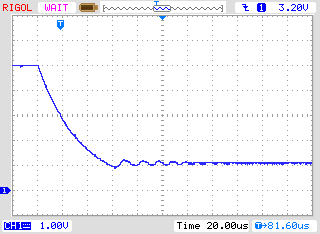
\includegraphics[width=.95\textwidth]{../PNG/AREF2_1V.png}
    \caption{od \(5V\) na \(1.1V\) }
    \label{pic:aref1}
  \end{subfigure}
  ~
  \begin{subfigure}[b]{.5\textwidth}
    \centering
    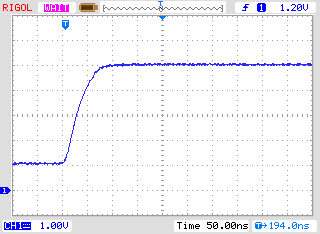
\includegraphics[width=.95\textwidth]{../PNG/AREF2VCC.png}
    \caption{z \(1.1V\) na \(5V\)}
    \label{pic:aref5}
  \end{subfigure}
  \caption{Přepnutí z AREF při použití \(1nF\) kondenzátoru}
\end{figure}

\begin{description} \setlength{\itemsep}{0em}
  \item[REF\_R\_KORR] určuje ofset vnitřního referenčního napětí v jednotkách mV.
S tímto ofsetem může být nastaven rozdíl v přepínání referenčního napětí při měření odporu.
Pokud byla vybrána volba AUTO\_CAL je tato hodnota pouze ofset k rozdílu napětí nalezenému ve
funkci AUTO\_CAL.\\
Příklad: CFLAGS += -DREF\_R\_KORR=10
  \item[OP\_MHZ] informuje software o tom, s jakou frekvencí v MHz bude tester pracovat.
Software je zkoušena pouze s \(1MHz\), \(8MHz\) a také s \(16MHz\).\\ Provoz s \(8MHz\) je pro lepší rozlišení
při měření kondenzátorů a cívek doporučen.\\
Příklad: OP\_MHZ = 8
  \item[RESTART\_DELAY\_TICS] musí být nastaven na 6, pokud je ATmega168 nebo ATmega328 v provozu
bez krystalu s RC Generátorem.
Pokud tato hodnota není přednastavena, zvolí software 16384 taktů zpoždění startu krystalové operace.\\
Příklad: CFLAGS += -DRESTART\_DELAY\_TICS = 6
  \item[USE\_EEPROM] určuje, zda mají být uloženy pevné texty a tabulky v paměti EEPROM.
V opačném případě se používá programová paměť (Flash).
Doporučuje se používat paměť EEPROM (možnost zvolená).\\
Příklad: CFLAGS += -DUSE\_EEPROM
  \item[EBC\_STYLE] označuje, že výstup přiřazení tranzistorových pinů by měl být ve
formátu  \inquotes{EBC=...} eventuálně. \inquotes{GDS=\dots}.
Tato prezentace šetří programový prostor.
Bez této volby bude přiřazení zobrazeno ve formátu \inquotes{123=\dots} kde každý bod může být E (emitor),
B (báze) nebo K (kolektor).
U FETs může být každý bod G (gate), D (drain) nebo S (source).
Pokud pořadí zkušebních čepů není v pořadí čtení 1,2 a 3,lze pomocí volby EBC\_STYLE=321 pořadí otočit.
Pak  bude přiřazení pinů ve tvaru \inquotes{321=\dots}, což je obvyklý směr čtení zleva doprava, což je vhodné,
 když mají zkušební kolíky pořadí 3,2,1.\\
Příklad: CFLAGS += EBC\_STYLE
  \item[NO\_NANO] označuje, že desetinná předpona Nano by neměla být použita k zobrazení výsledků měření.
Kapacitní hodnoty jsou uvedeny v \(\mu F\) místo \(nF\).\\
Příklad: CFLAGS += NO\_NANO
  \item[NO\_LONG\_PINLAYOUT] lze nastavit, aby se zabránilo dlouhé podobě pinout na grafických displejích
jako \inquotes{ Pin  1=E 2=B 3=C}.
Je-li volba nastavena, použije se krátká forma jako \inquotes{ Pin  123=EBC}.\\
Example: CFLAGS += NO\_LONG\_PINLAYOUT
  \item[PULLUP\_DISABLE] znamená, že nepotřebujete vnitřní \inquotes{Pull-Up} odpory.
Musíte mít externí \inquotes{Pull-Up} odpor pro Pin 13 (PD7) a VCC zapojený, k použití této volby.
Tato možnost zabraňuje možnému ovlivnění \inquotes{Pull-Up} odporů na měřících portů (Port B a Port C).\\
Příklad: CFLAGS += -DPULLUP\_DISABLE
  \item[ANZ\_MESS] Tato volba určuje, jak často má být hodnota ADC čtena a přidána.
Můžete zvolit hodnotu mezi 5 a 200, abyste získali průměrnou hodnotu pro měření ADC.
Vyšší hodnoty poskytují větší přesnost, ale měřitelnost trvá déle.
Měření ADC s hodnotou 44 potřebuje asi \(5ms\).\\
Příklad: CFLAGS += -DANZ\_MESS=44
  \item[POWER\_OFF] Tato funkce zapíná funkci automatického vypnutí.
Pokud tuto možnost vynecháte, měření v smyčce se opakují nekonečně až do přerušení provozního napětí.
Pokud máte tester s vypínačem místo spínacích tranzistorů, můžete tuto možnost vynechat.
Pokud vynecháte volbu POWER\_OFF, existuje přesto možnost vypnutí, pokud jste zvolili možnost WITH\_MENU.
Můžete také použít volbu POWER\_OFF pro zadání počtu měření, po kterých se tester vypne,
když nenalezne žádnou vloženou součástku.
S dvojnásobným počtem po sobě jdoucích měření s nalezenou komponentou se tester také vypne,
pokud není mezi nimi, měření bez nalezené součástky.
Pokud zapomenete vyjmout připojenou součástku, zabrání to úplnému vybití baterie.
Specifikace doplňku ve tvaru  CFLAGS += -DPOWER\_OFF=5 po 5ti, po sobě jdoucích měření bez
nalezené součástky, také vypne.
Následujících 10 měření s nalezenou součástkou vypne také.
Pouze v případě, že příslušné měřicí řady jsou přerušeny jiným typem, měření pokračuje.
Výsledky měření pro jedno měření se zobrazují po 28 sekund, pro více měření se
čas zobrazení sníží na 5 vteřin (nastaveno v config.h).
Pouze pokud se při prvním startu tlačítko start dlouze stiskne, zobrazí se výsledek měření
také pro řadu postupných měření po dobu 28 vteřin.
Maximální hodnota opakování je 255 (CFLAGS += -DPOWER\_OFF=255).\\
Příklad 1: CFLAGS += -DPOWER\_OFF=5 \\
Příklad 2: CFLAGS += -DPOWER\_OFF 
  \item[BAT\_CHECK] zapne kontrolu napětí baterie.
  Pokud tuto možnost nezadáte, zobrazí se číslo verze softwaru.
Tato volba je užitečná pro upozornění na změnu baterie na testerových verzí s baterií.\\
Příklad: CFLAGS += -DBAT\_CHECK
  \item[BAT\_OUT] zapne indikátor napětí baterie na displeji LCD, když je vybrána položka BAT\_CHECK.
 Je-li vaše napájecí zdroj \(9V\)  vybaven diodou pro ochranu proti přepólování, můžete
zadejte formu BAT\_OUT=600 na prahovou hodnotu diodového prahu
které je třeba vzít v úvahu v zobrazení napětí.
V této možnosti lze také zvážit ztrátu napětí na tranzistoru T3.
Specifikace prahového napětí v mV nemá vliv na hodnoty zkušebního napětí (BAT\_POOR).\\
Příklad 1: CFLAGS += -DBAT\_OUT=300 \\
Příklad 2: CFLAGS += -DBAT\_OUT
  \item[BAT\_POOR]  nastaví prázdné napětí pro test napětí baterie na zadanou hodnotu v jednotkách \(1mV\).
Výstražné napětí je \(0,8V\) vyšší než zadané prázdné napětí, když je prázdné napětí větší než \(5,3V\).
V opačném případě bude vybráno \(0,4V\) vyšší výstražné napětí,
pod \(3,25V\) dokonce pouze jedno \(0,2V\) vyšší výstražné napětí pod \(1,3V\) pouze
jedno \(0,1V\) vyšší výstražné napětí než specifikované prázdné napětí.
Nastavování prázdného napětí na hodnoty jako \(5,4V\) se nedoporučuje u dobíjecích
baterií \(9V\),protože zvyšuje riziko poškození baterie v důsledku hlubokého vybití!
Používáte-li dobíjecí baterie \(9V\) doporučují se typy \inquotes{Ready to Use} z důvodu nižšího samovybíjení.\\
Příklad ovládacího prvku low-drop (\(5,4V\)): CFLAGS += -DBAT\_POOR=5400 \\
Příklad regulátoru 7805 (\(6,4V\)): CFLAGS += -DBAT\_POOR=6400
  \item[DC\_PWR] Tato úroveň napětí v jednotkách mV určuje výše uvedený limit napětí baterie
který se změní na \inquotes{DC\_Pwr\_Mode}.
Tester obvykle běží v režimu baterie, kde všechny další funkce běží po omezenou dobu.
Pomocí funkce \inquotes{DC\_Pwr\_Mode} se doplňkové funkce provádějí neomezeně.
Protože neexistuje měnič DC-DC se vstupním napětím \(0.9V\),
\inquotes{DC\_Pwr\_Mode} se také spustí, pokud je detekováno napětí baterie pod  \(0.9V\).\\
Příklad: CFLAGS += -DDC\_PWR=9500
 \item[BAT\_NUMERATOR] Definuje čitatel zlomku, se kterým musí být vyhodnoceno vnější napětí,
abyste získali správné napětí.
Pro standardní dělič napětí s \(10 k\Omega\) a \(3.3 k\Omega\) odpor je kvocient (10000 + 3300)/3300.
Koeficient získaný pomocí hodnot odporu by měl být zkrácen. Například výsledky 133/33 .\\
Příklad: CFLAGS += -DBAT\_NUMERATOR=133
 \item[BAT\_DENOMINATOR] Určuje jmenovatele zlomku, se kterým musí být vyhodnoceno externí napětí.\\
Příklad: CFLAGS += -DBAT\_DENOMINATOR=33
 \item[EXT\_NUMERATOR] Definuje čitatel zlomku, se kterým musí být vyhodnoceno vnější napětí.
abyste získali správné napětí. Pro standardní dělič napětí s \(180 k\Omega\) a \(20 k\Omega\) odpor
je kvocient (180000+20000)/20000.
Kvocient by měl být zkrácen na 10/1.\\
Příklad: CFLAGS += -DEXT\_NUMERATOR=10
 \item[EXT\_DENOMINATOR] Určuje jmenovatele zlomku, se kterým musí být vyhodnoceno vnější napětí.\\
Příklad: CFLAGS += -DEXT\_DENOMINATOR=1
  \item[INHIBIT\_SLEEP\_MODE] zakáže použití režimu spánku procesoru.
Normálně software používá spánkový stav procesoru pro delší pauzy, aby šetřil energii.
Použití tohoto stavu spánku s probuzením šetří kapacitu baterie,
představuje další požadavek pro regulátor napětí.\\
Příklad: DINHIBIT\_SLEEP\_MODE=1
  \item[PROGRAMMER] \label{PROGRAMMER} nastavuje typ programátoru pro program rozhraní '\lcmd{avrdude}'.
Bez správného nastavení použitého programátoru '\lcmd{avrdude}' nefunguje.
Standardně je připravený programátor firmy Diamex.
Připraveny jsou, USBasp firmy Fischler a Arduino mega.
Používáte-li jiný programátor, musíte ho přidat, a ten připravený pomocí \#~odhlásit.
Příklad pro použití USBtiny programátoru:
\vspace{-1\baselineskip}
\begin{verbatim}
# setting for USBtiny ISP
PROGRAMMER=usbtiny
BitClock=10
PORT=usb
Další příklad přidání, Programátor od firmy Pololu:
#~setting for Pololu programmer
#~PROGRAMMER=stk500v2
#~BitClock=1.0
#~PORT = /dev/ttyACM0
\end{verbatim}
Příklad: PROGRAMMER=avrisp2
  \item[BitClock] nastavuje dobu taktové periody pro programátora. Viz popis parametru -B avrdudu.\\
Příklad: BitClock=5.0
  \item[PORT] nastavuje použité rozhraní, kde může \lcmd{avrdude} dosáhnout mikrokontroléru (ATmega).\\
Příklad: PORT=usb
\end{description}

Další informace naleznete v příručce pro \lcmd{avrdude} nebo v online dokumentaci~\cite{avrdude}.
Další parametry lze nastavit v souborech Transistortester.h a config.h.
Soubor config.h obsahuje globální proměnné a tabulky, definuje souhvězdí port / pin,
frekvenci hodin ADC a hodnoty odporu použité pro měření.
Soubor Transistortester.h obsahuje globální proměnné a tabulky, jakož i texty pro LCD displej.
Obvykle se tyto hodnoty nemusejí bez důvodu změnit.
\section{Programování mikrokontroléru}
Vydávám software pro mikrokontrolér ve zdrojovém kódu.
Vývoj byl proveden s operačním systémem Linux (Ubuntu přesněji Mint) a je ovládán přes \lname{Makefile}.

\lname{Makefile} zajišťuje, že software je stejný jako v souboru \lname{Makefile} předem zvolené možnosti.
Podívejte se prosím do souboru Readme.txt
v adresáři trunk/default a v kapitole~\ref{sec:config} od strany~\pageref{sec:config}.

Výsledkem překladu jsou soubory s příponou .hex a .eep.
Obvykle se soubory nazývají TransistorTester.hex a TransistorTester.eep.\\
Soubor .hex obsahuje data pro programovou paměť (Flash) procesoru ATmega.
Soubor .eep obsahuje údaje pro EEPROM ATmega.
Oba soubory musí být načteny do správné paměti.

Navíc ATmega musí být správně nakonfigurována s pojistkami (fuses).
Pokud používáte \lname{Makefile} spolu s programem \lcmd{avrdude} \cite{avrdude}, nepotřebujete mít
žádné přesné znalosti o detailech pojistek.
Musíte volat pouze \lcmd{make fuses}, pokud nepoužíváte krystal nebo,
pokud máte na desce nainstalovaný  \(8MHz\) krystal, musíte zvolit \lcmd{make fuses-crystal}.
S řadou mikrokontrolérů ATmega168 můžete alternativně zvolit \lcmd{make fuses-crystal-lp} pro
provoz s nízkou spotřebou krystalu.
Nikdy nepoužívejte verzi pro krystal, pokud nemáte v použití \(8MHz\) krystal.
Pokud si nejste jisti, nechte nejdříve tovární nastavení v  a spusťte testovací přístroj v tomto stavu.
Je možné, že program běží příliš pomalu, ale to můžete později opravit!
Když ale použijete programovou versi pro \(8MHz\) krystal, 
tak nesprávné nastavení pojistky může zabránit pozdějšímu ISP programování.

\subsubsection{Poznámka překladatele}
\label{linux}
aby zůstalo všem ostatním kolegům zoufalství a "`bezesné nocí"' ušetřeno, kterými trpěl autor této kapitoly, poté co získal klone testeru a bez jakékoli zkušenosti s AVR se rozhodl, ho "`naučit česky"', vznikla tato kapitola. Získané zkušenosti by měly pomoci všem ostatním naivním,\\ "`ochotným \dots lehkomyslným a nezkušeným"'\dots, ÚSPĚŠNĚ naprogramovat jejich tester.
\\
Tato příležitost je zároveň využita, poděkovat autorovi a vývojáři tranzistorového testeru
Karlovi-Heinzy Kübbelerovi viz \cite{karlheinz1} za jeho obětavost a trpělivost, protože bez jeho pomoci, by následující stránky nebyly napsány.
     
Aby překlad firmwaru a vypálení do MCU uspělo a současně \dots
"`nemuselo být "`kolo"' znovu objeveno"', je část následujících stránek převzatá z originálu.

Tak ještě jednou \dots \huge{MOC VELKÝ VDĚK}.
\normalsize
\subsection{Operační system Linux}
Programování pod Linuxem přináší mnoho výhod, protože tento OS byl vyvinut odborníky, kteří se orientují  přáním uživatelů.\\
Prostředí je navíc k dispozici zdarma a je dokonale udržováno.
Další výhodou je zabezpečení samotného operačního systému, hlavně při používání internetu.
Jak používání, tak i instalace dnešních vydání je mnohem jednodušší než u konkurenčních operačních systémů.\\
Existují také velmi výkonné editory, jako jsou "`vim"' nebo "`emacs"', které ale vyžadují trochu času k zapracování. Zejména "`Vim"' má tu výhodu, že
je předinstalován v každém systému a je také dostupný i u ostatních OS včetně Windows. Ale právě u tohoto editoru vyžaduje přepínání, mezi režimem zadávání a režimem příkazů, zvyk a tréning. 

Tento tutoriál je tak navržen, aby povzbudil všechny "`ne"' uživatele Linuxu, aby se o tom, naprogramováním svého testeru v Linuxu, přesvědčili.
Jako příklad, je zde použitý Linux Mint cinnemon v aktuální verzi, která je bezplatně k dispozici na internetu.  
Instalace je možná na různé způsoby, Linux přinese svého spouštěcího asistenta, který se samostatně předchozí OS respektuje a nakonfiguruje
Linux k paralelnímu použití.
\vspace*{-0.3cm} 
\subsubsection{Rady k použití s Linuxem}
Pro ty, kteří neradi píší, nabízí Linux snadný způsob, jak si to ulehčit.
Zkopíruj tuto příručku na USB klíčenku a otevři ji dvojitým zmáčknutím levým tlačítkem myši \LMB na tvém desktopu.
Alternativně k dvojitému zmáčknutí můžeš pravým tlačítkem \RMB zvolit jiný, než předvolený prohlížeč PDF.   
Poté přesuň myš na název dokumentu, stiskni levé \LMB myší tlačítko a táhni dokument k levému okraji obrazovky, až se zobrazí možný rámeček. Nyní  myš uvolni.
Příručka nyní zabere levou polovinu obrazovky.
 
Jak je pro Linux typické, existuje další řada možností ke změně velikosti dokumentu. S levým tlačítkem \LMB na okrajích nebo rozích okna, 
nebo pravým tlačítkem \RMB na hlavové liště pomocí funkce \menu[,] {{změnit velikost}}.
Operace je jinak stejná jako při posunu.

Grafická rozhraní v systému Linux mají zpravidla více než jednu pracovní plochu,
s kombinací kláves \keys{{Ctrl} + \ Alt + \arrowkeyright}
nebo \keys{{Ctrl} + \ Alt + \arrowkeyleft} je lze přepnout.
Pomocí pravého tlačítka \RMB můžeš zadat a vybrat pracovní prostor, na kterém je okno zobrazeno.

Okna, která potřebuješ pro aktuální práci, můžeš mít tedy na pracovní ploše shromážděné a nedusíš se ve všech oknech pro různé pracovní oblasti.
Mimochodem, se všemi položkami příkazů a identifikátory souborů je důležité vědět, že Linux konsekventně rozlišuje velká a malá písmena.
\vspace*{-0.3em}  
\subsubsection{Instalace programových balíčků}
\label{paket}
K naprogramování testeru, musíš nejprve stáhnout s internetu a nainstalovat programové balíčky:

 binutils-avr, avrdude, avr-libc, gcc-avr a git.
 To docílíš následovně. Naviguj ve tvé příručce k na tuto stránku~\pageref{paket} k následujícímu textu:

\begin{large} \vspace{-0.4em} \begin{verbatim}
sudo apt-get install avrdude avr-libc binutils-avr gcc-avr git
\end{verbatim} \end{large}
 
Nyní současně stiskni \keys{{Strg} + \Alt + t} k otevření příkazového okna, které již známým způsobem přesuneš, nyní na pravou polovinu obrazovky. 
Příručka nyní zabere levou polovinu obrazovky.\\
V dalším kroku označ levým myším tlačítkem \LMB ten výše jmenovaný text v levém okně. Při dosáhnutí posledního písmene, povol tlačítko k ukončení označení.
Je-li text ve vlastním řádku, jako v tomto případě, je možné ho označit trojitým zmáčknutím levého tlačítka \LMB v jeho řádku.

Přesuň nyní myš na kurzor v pravém příkazovém okně a vlož tento text stisknutím prostředního tlačítka myši, \textbf{dále zkráceně \MMB} do okna terminálu.
U většiny myší je rolovací kolečko také prostředním tlačítkem.
U myší bez prostředního tlačítka je možné napodobit prostřední tlačítko myši současným stisknutím tlačítek \LRMB.
Bez ohledu na to, jak se text příkazu dostal do příkazového řádku, by jsi měl tento text zkontrolovat, než odešleš tento příkaz stisknutím klávesy
 \keys{\enter}.
S instalací balíčků si obvykle nemusíš dělat starosti, že se, kvůli nesprávné operaci, stane něco špatného.
Program \lcmd{apt-get} zkontroluje, zda některý z uvedených balíčků není již nainstalovány a zda jsou nutné závislosti splněny.
V případě potřeby bude, již dříve nainstalovaný balíček, nahrazen novějším.
Poté vás program \lcmd {sudo} nejprve požádá o uživatelské heslo, než to udělá zbytek příkazového řádku.
Heslo byste měli vyplnit a potvrdit stisknutím klávesy \keys{\enter} nebo \keys {\return}.
Nyní budou všechny softwarové balíčky staženy a nainstalovány programem \lcmd{apt-get}.

Je možné, že se \lcmd{apt-get} při instalaci balíčků ptá na detaily, na které lze obvykle potvrdit.   
\\ \textbf{*Pozor,} Linux rozlišuje mezi malými a velkými písmeny. Takže odpovídej s \keys{J} a ne s \keys{j}~!

Samozřejmě existují i ​​jiné způsoby instalace balíčků, které používají grafické uživatelské rozhraní
jako \lcmd{synaptic} nebo \lcmd{dpkg}. Ale není jednodušší způsob instalace smíšených skupin balíčků. 
\vspace*{-0.3em} 
\subsubsection{Stáhnutí zdrojů}
Zda byla instalace správce zdrojů Github úspěšná, lze kontrolovat s:
\begin{large} \vspace{-0.4em} \begin{verbatim}
git version
\end{verbatim} \end{large}
Jako odpověď se ukáže číslo instalované verse.\\ 
Pokud složka transistortester již existuje, měla by být nyní přejmenována nebo odstraněna. \\
Příkazem:

\begin{large} \vspace{-0.4em} \begin{verbatim}
git clone https://github.com/Mikrocontroller-net/transistortester
\end{verbatim} \end{large}
stáhneš celý archiv. \\
Soubory jsou nyní v Linuxu [osobní složka] na \lname{/home/"`uživatel"'} pod názvem \inquotes{transistortester}.\\
Kontrolu přítomnosti docílíš, když v okně terminálu, zadáš \lcmd{ls} to je \(\mbox{\keys{l} \keys{s} \keys{\return}}\)~.\\
Více informací o souborech a adresářích získáš pomocí
příkazu \lcmd{ls -lh}. Zde byly kombinovány dvě možnosti příkazu \lcmd{ls}
a k tomu možnosti \lcmd{{-l}} a \lcmd{{-h}}. Tento vstupní formulář je tedy krátký formulář pro
příkaz \lcmd{ls -l -h} nebo \lcmd{ls -l --lidsky čitelný}.
Některé možnosti přicházejí ve dvou verzích, krátká s - (\lcmd{{-h}})
a dlouhý formulář se dvěma - (\lcmd{{--human-readable}}).
Mimochodem, na pořadí možností nezáleží,
stejně jako počet oddělovacích mezer \keys{\space}.
S téměř všemi příkazy se můžete dozvědět více o operaci a možnostech
přidáním možnosti \lcmd{{--help}}.
To samozřejmě platí i pro příkaz \lcmd{git}. \\ 
Chceš-li v budoucnu stáhnout nové aktualizace, postačí z této složky zadat:
\begin{large} \vspace{-0.4em} \begin{verbatim}
git pull
\end{verbatim} \end{large}
v okně terminálu a v pracovním adresáři \lname{"`transistortester"'}~,
nebo z jakéhokoliv adresáře s:

\begin{large} \vspace{-0.4em} \begin{verbatim}
(cd ~/transistortester ; git pull)
\end{verbatim} \end{large}

K zajištění správné funkce výzvy \lcmd{git pull} , se doporučuje, neměnit adresářový strom. 

\subsubsection{Používání USB rozhraní}
Všechny moderní ISP nástroje k programování se sériovým rozhraním používají USB,
protože toto rozhraní také zajišťuje napájení.
U těchto zařízení by jsi měl jako prvé zkontrolovat, jaké označení je přiřazené k tomuto zařízení.
Při vložení nástroje do USB zásuvky v systému Linux je vytvořen záznam do systémového protokolu.
Protože je systémový protokol textový soubor, nechá se jednoduše zobrazit na obrazovce.
Chceš-li to provést, můžeš použít příkaz \lcmd{dmesg} v okně terminálu.
A proto, že nás, po zastrčení nástroje zajímají pouze na poslední řádky protokolu, použij:

\verb"dmesg|tail"\\
Program \lcmd{dmesg} zobrazuje celý systémový protokol a příkaz
\lcmd{tail} zobrazuje pouze posledních 10 řádků výstupu.
U programátoru \lname{Pololu} vypadá výsledek takto:
\vspace*{-.5em}
\begin{footnotesize} \begin{verbatim}
usb 1-3: new full-speed USB device number 3 using xhci_hcd
usb 1-3: New USB device found, idVendor=1ffb, idProduct=00bb, bcdDevice= 1.02
usb 1-3: New USB device strings: Mfr=1, Product=2, SerialNumber=3
usb 1-3: Product: Pololu USB AVR Programmer v2.1
usb 1-3: Manufacturer: Pololu Corporation
usb 1-3: SerialNumber: 00227484
cdc_aem 1-3:1.1: ttyACM0: USB ACM device
cdc_aem 1-3:1.3: ttyACM1: USB ACM device
usbcore: registered new interface driver cdc_acm
cdc_aem: USB Abstract Control Model driver for USB modems and ISDN adapters
\end{verbatim} \end{footnotesize}
\vspace*{-.5em}
Zde jsou důležité řádky 7 a 8 se vstupy ttyACM0 a ttyACM1.
Jedná se o přiřazené názvy zařízení pro dvě sériová rozhraní.
V Linuxu jsou všechna zařízení také součástí stromu souborů a jsou v
souboru \lname{/dev/} registrované. Přiřazené Jméno nástroje \lname{Pololu} se skládá
z dvou sériových rozhraní, a to \lname{/dev/ttyACM0} a \lname{/dev/ttyACM1}.
U programátora  \lname{Pololu} musíš vědět, že první sériové rozhraní
se používá pro ISP programátor a druhé sériové rozhraní
lze volně použít pro jiné účely.\\
Existenci položek zařízení můžeš potvrdit pomocí příkazu:
\begin{large} \vspace{-0.4em} \begin{verbatim}
ls -l /dev/ttyACM*
\end{verbatim} \end{large}
Výsledek by měl vypadat takto: 
\begin{footnotesize} \begin{verbatim}
crw-rw---- 1 root dialout 166, 0 Mär 11 09:57 /dev/ttyACM0
crw-rw---- 1 root dialout 166, 1 Mär 11 09:57 /dev/ttyACM1
\end{verbatim} \end{footnotesize}
V tomto výstupu se dozvíš, že pro toto zařízení může ovládat uživatel \lname{root}
a je použití je povoleno pro skupinu uživatelů \lname{dialout} .
Tvé členství v této skupině můžeš zkontrolovat pomocí příkazu:

\verb"id"\\
V odpovědi by se v seznamu měla objevit skupina \lname{dialout} .
Přístup ke členství do skupiny je popsán níže v dalším pracovním bodě.
Předtím ale další příklad systémového protokolu pro nástroj jiného
ISP-programátora  \lname{Diamex ISP-PRog NG} si můžeš prohlédnout zde: 
\vspace*{-.5em}
\begin{footnotesize} \begin{verbatim}
usb 1-6: new full-speed USB device number 8 using xhci_hcd
usb 1-6: New USB device found, idVendor=16c0, idProduct=2a9b, bcdDevice=43.40
usb 1-6: New USB device strings: Mfr=1, Product=2, SerialNumber=3
usb 1-6: Product: AVR-ISP2
usb 1-6: Manufacturer: ERFOS
usb 1-6: SerialNumber: 19377-43111-757
cdc_aem 1-6:1.0: ttyACM0: USB ACM device
\end{verbatim} \end{footnotesize}
\vspace*{-.5em}
Přehled připojených sériových převodníků USB jze vidět v adresáři \lname{/dev/serial/by-id/},
které lze dotazovat příkazem:

\verb"ls -og /dev/serial/by-id/* | cut -d' ' -f 7-"\\ 
Výstup může například vypadat takto:
\vspace*{-.2em} 
\begin{footnotesize} \begin{verbatim}
/dev/serial/by-id/usb-Arduino__www.arduino.cc__0043_954323131383519062F0-if00 -> ../../ttyACM2
/dev/serial/by-id/usb-Pololu_Corporation_Pololu_USB_AVR_Programmer_v2.1_00227484-if01 -> ../../ttyACM0
/dev/serial/by-id/usb-Pololu_Corporation_Pololu_USB_AVR_Programmer_v2.1_00227484-if03 -> ../../ttyACM1
\end{verbatim} \end{footnotesize}
\vspace*{-.2em}
Pokud je popis dostatečně podrobný, můžete tímto způsobem přiřadit rozhraní.

Pokud je, až k tomuto bodu vše v pořádku, je třeba změnit v \lname{Makefile} pouze položku PORT 
za \inquotes{PORT=/dev/ttyACM0},
aby měl program \lcmd{avrdude} přístup k programátorovi.
Pokud se ve tvém systému používají jiná USB sériová rozhraní, mohou se v označení zařízení poslední číslice lišit.
Chtěl bych také zmínit o další skupině USB-serial rozhraní která používá místo \lname{ttyACM} název \lname{ttyUSB}.

Pokud tvůj programátor používá speciální USB rozhraní ale
žádný sériový typ USB, je pravděpodobně nutná další práce. V \lname{Makefile} můžeš nastavit PORT pevně na \lname{USB}. 
Ale je pravděpodobné, že stejně budeš mít přístup k zařízení.
Všechna připojená USB zařízení lze zobrazit zadáním \lcmd{lsusb} do příkazového okna. Zadej:

\verb"lsusb"\\
před a po připojení tvého USB programátora.
Porovnáním výsledků tento nástroj lokalizuješ. Výsledek může vypadat takto:
\vspace*{-.6em}
\begin{footnotesize} \begin{verbatim}
Bus 001 Device 001: ID 1d6b:0002 Linux Foundation 2.0 root hub
Bus 002 Device 003: ID 046d:c050 Logitech, Inc. RX 250 Optical Mouse
Bus 002 Device 058: ID 03eb:2104 Atmel Corp. AVR ISP mkII
Bus 002 Device 059: ID 2341:0042 Arduino SA Mega 2560 R3 (CDC Aem)
Bus 002 Device 001: ID 1d6b:0001 Linux Foundation 1.1 root hub}
\end{verbatim} \end{footnotesize}
\vspace*{-.6em}
Zde bylo detekováno zařízení AVR ISP mkII jako zařízení 58 \lname{DIAMEX ALL-AVR}.\\
ID 03eb je jeden ID výrobce a ID 2104 identifikátor produktu.\\
Tyto dva identifikátory je nutné zapsat do souboru /etc/udev/rules.d/90-atmel.rules pomocí:

\verb"sudo xed /etc/udev/rules.d/90-atmel.rules"\\
Pochopitelně je možné,použít také jiný editor než \lname{xed}. 
V tomto příkladu obsahuje soubor 90-atmel.rules pouze jeden řádek:
\vspace*{-0.6em}
\begin{footnotesize}\begin{verbatim}
SUBSYSTEM=="usb", ATTRS{idVendor}=="03eb", ATTRS{idProduct}=="2104", MODE="0660", GROUP="plugdev"
\end{verbatim} \end{footnotesize}
\vspace*{-0.6em}
Záznam je v Linuxu také možné vytvořit i bez editoru pomocí příkazu:
\begin{footnotesize} \vspace{-0.4em} \begin{verbatim}
sudo echo 'SUBSYSTEM=="usb", ATTRS{idVendor}=="03eb", ATTRS{idProduct}=="2104"
, MODE="0660", GROUP="plugdev"' >> /etc/udev/rules.d/90-atmel.rules
\end{verbatim} \end{footnotesize}
Zde viditelné dva řádky je nutné zapsat v terminálu jako JEDEN řádek!\\
 Pro použití většiny programátorů se doporučuje napsat do 90-atmel.rules následující text,
který je nutné tak upravit, aby stál celý příkaz vždy v jednom řádku
(jako je to již u \#~Pololu programátoru):
\vspace*{-1em}
\begin{footnotesize} \begin{verbatim}
# Copy this file to /etc/udev/rules.d/90-atmel.rules
# AVR ISP mkII- DIAMEX ALL-AVR
SUBSYSTEM=="usb", ATTRS{idVendor}=="03eb", ATTS{idProduct}=="2104", GROUP="plugdev",
 MODE="0660"
# Atmel AVR Dragon
ATTRS {idVendor}=="03eb", ATTRS {idProduct}=="2107", GROUP="plugdev", MODE="0660"
# Atmel-ICE
SUBSYSTEM=="usb", ATTRS {idVendor}=="03eb", ATTRS {idProduct}=="2141", GROUP = "plugdev",
 MODE="0660",
# xplained-mini
SUBSYSTEM=="usb", ATTRS {idVendor}=="03eb", ATTRS {idProduct}=="2145", GROUP = "plugdev",
 MODE="0660",
# avrftdi
#SUBSYSTEM=="usb", ATTRS {idVendor}=="0403, ATTRS {idProduct}=="6010", GROUP = "plugdev",
 MODE="0660",
# UM232H
#SUBSYSTEM=="usb", ATTRS {idVendor}=="0403, ATTRS {idProduct}=="6014", GROUP = "plugdev",
 MODE="0660",
# USBasp programmer for Atmel AVR controllers FISCHL
ATTRS{idVendor}=="16c0", ATTRS{idProduct}=="05dc", GROUP="plugdev", MODE="0660"
# USB NIBObee-Programmer
ATTRS {idVendor}=="16c0", ATTRS {idProduct}=="092f", GROUP="plugdev", MODE="0660"
# USBtiny ISP programmer
ATTRS{idVendor}=="1781", ATTRS{idProduct}=="0c9f", GROUP="plugdev", MODE="0660"
# USB ISP-programmer für Atmel AVR
SUBSYSTEM=="usb", ENV {DEVTYPE}=="usb_device", SYSFS {idVendor}=="16c0", SYSFS {idProduct}
 == "05dc", MODE="0660",
\end{verbatim} \end{footnotesize}
Po zapsání lze svůj úspěch kontrolovat s:
\begin{footnotesize} \vspace{-0.4em} \begin{verbatim}
less /etc/udev/rules.d/90-atmel.rules
\end{verbatim} \end{footnotesize}
Pak bys měl systém pžimět k tomu, aby znovu načetl pravidla udev pomocí: 
\begin{footnotesize} \vspace{-0.4em} \begin{verbatim}
sudo udevadm control --reload-rules
\end{verbatim} \end{footnotesize}
a kromě toho, ještě svůj ISP programátor odpojit a znovu ho připojit. 
To umožňuje přístup k zařízení pro členy skupiny \lname{plugdev}.
K dispozici bylo také rozpoznáno zařízení 59 USB Arduino Mega 2560 SA systém, které vytváří přístup
k sériovému zařízení \inquotes{/dev/ttyACM0} pro členy skupiny \lname{dialout}.
\vspace*{-0.3em} 
\subsubsection{Skupinové členství}
pro tvé vlastní uživatelské jméno, ve skupinách \lname{plugdev} i \lname{dialout} dosáhneš přikazem:
\begin{large} \vspace{-0.4em} \begin{verbatim}
sudo usermod -a -G dialout,plugdev $USER
\end{verbatim} \end{large}
Nyní by měl být možný přístup s \lcmd{avrdude}m k oběma zařízení.
Kontrola je možná zadáním:
\lcmd{id}\\
Pokud by se vyskytly problémy, můžeš také přistoupit k členství prostřednictvím: \\
~ \menu[,]{Nabídka menu,{Správa systému},{Uživatelé a skupiny},{?heslo}}. Zobrazí se okno se dvěma záložkami. \\
Pokud nyní klikneš na své jméno na kartě uživatelé, uvidíš svůj profil a skupinové přidružení na pravé straně. Pomocí tlačítka \menu[,]{ADD} je nyní možné, přidat nové skupiny.\\
Nabídku menu lze lehce dosáhnout s \keys{\winmenu} to je tlačítko mezi \keys{{Strg}} a \keys{\AltGr} na pravé straně klávesnice.
\vspace*{-0.3em} 
\subsubsection{Příprava pracovního prostředí} 
Terminálové okno se otvírá normálně v domovském adresáři \lname{../home/user}.
Název tvého domovského adresáře je uložen v systémové proměnné \lname{\$HOME}.
Do tohoto adresáře se dostaneš v terminálu z jakéhokoli adresáře také krátkým povelem:

\verb"~/"\\
Nezapomeň zadat po zadání \lname{\textasciitilde} zadat také znamení \lname{/} , jinak hledá tlumočník příkazů uživatele s následujícím jménem!\\   
Aby zůstal originál čistý je výhodné vytvořit duplikát svého testeru v pracovním adresáři se jménem například \lname{\textbf{Mytester}}.\\
Nejprve vytvoříš nový Adresář s povelem:
\begin{large} \vspace{-0.4em} \begin{verbatim}
mkdir ~/Mytester
\end{verbatim} \end{large}

Pokud jsi stáhl z \lname{Github} archivu všechny zdrojové soubory do adresáře \lname{\textasciitilde/transistortester},\\
získáš následujícím příkazem kopii tvých souborů a jejich podadresářů do adresáře \lname{\textbf{Mytester}}: 
\begin{large} \vspace{-0.4em} \begin{verbatim}
rsync -auv ~/transistortester/Software/trunk ./Mytester
\end{verbatim} \end{large}

Kvůli přítomnosti \lcmd{-v} protokoluje \lcmd{rsync} všechny procesy kopírování.
Pokud místo možností \lcmd {-auv} zadáš jen \lcmd{-au}, proces kopírování nezaznamenává.
K naplněnému kufru podadresáře však můžete přistupovat pomocí následujícího příkazu
přesvědčit: 
\begin{large} \vspace{-0.4em} \begin{verbatim}
ls -lh ~/Mytester/trunk
\end{verbatim} \end{large}

K dispozici je také jasná reprezentace adresářové struktury a souborů příkazem:
\begin{large} \vspace{-0.4em} \begin{verbatim}
tree ~/Mytester
\end{verbatim} \end{large}

Tento příkaz \lcmd{tree}není ale standardně instalovaný. Pomocí:
\begin{large} \vspace{-0.4em} \begin{verbatim}
sudo apt-get install tree
\end{verbatim} \end{large}

ho můžeš ale lehce doinstalovat.

Pokud nyní víš, který podadresář je pro tvůj tester vhodný, můžeš přejít do tohoto podadresáře.\\
Příklad: máš čínskou sadu s černobílým displejem, pak je podadresář \lname{mega328\_st7565\_kit} správný
a zadáním:
\begin{large} \vspace{-0.4em} \begin{verbatim}
cd ~/Mytester/mega328\_st7565\_kit
\end{verbatim} \end{large}

Nyní nech okno terminálu otevřené a zkus otevřít tento Soubor následujícím způsobem:
\vspace*{-0.3em}   
\subsubsection{Příprava svého testeru pomocí grafické cesty}
\lname{\textbf{Mytester}} můžeš také dosáhnout dalšími způsoby.
Posuň myš na zelenou ikonou \lname{pořadač (Nemo)}  na systémové liště s nápisem \lname{Soubory}, nebo otevři \menu[,]{Nabídka} a napiš do výběrového okna začáteční písmena tvého účelu. V tomto případě stačí \menu[,]{so}, abys viděl \lname{Soubory} napravo. Kromě toho lze použít  také \menu[,]{Nabídka, Příslušenství, Soubory}. Dvojitým stiskem \LMB tvojí volbu otevři. Otevře se okno se všemi možnými testery a mezi nyní i vybraná složka \lname{mega328\_st7565\_kit} a v ní soubor \lname{Makefile}.
\vspace*{-0.3em} 
\subsubsection{Úprava Makefile}
Postav myš na tento soubor a dvojitým stiskem \LMB se otevře tento dokument s předvoleným editorem. Druhá možnost je stisknutí \RMB kdy se otevře menu
s různými možnostmi spravování. A pro ty, kterým se práce s terminálem zalíbila stačí zadat v terminálu:
\verb"xed Ma" dále \keys{{Tab}} a na konec \keys{\return}\\

Je jedno jakou cestou jsi se sem dostal, \textbf {v souboru \lname{Makefile} je nejdůležitější správně} zvolit tvůj USB programátor.
Více o tom v Kapitole \ref{PROGRAMMER} na stránce \pageref{PROGRAMMER}, bod PROGRAMMER.\\
Dále zde můžeš nastavit další možnosti jako řeč, písmo atd.
\vspace*{-0.3em} 
\subsubsection{Programování testeru}
A je čas se dostat k programování. Propoj svůj programátor s testerem a přes USB s počítačem.
Po té, co jsi tvé změny v \lname{Makefile} provedl, zkontroloval a dokument uložil, přejdi myší na okno terminálu a aktivuj ho stiskem na \LMB.
Aktivní okno poznáš tím, že má záhlaví vyšší kontrast!\\
Nyní stačí zadat příkaz:
\begin{large} \vspace{-0.4em} \begin{verbatim}
make upload
\end{verbatim} \end{large}

Tester program bud nyní znovu sestaven a poté okamžitě načten do ATmega \lcmd{avrdude} programem.
Nyní můžeš okamžitě tvůj úspěch zkontrolovat a oslavit.\\
V případě nespokojenosti, je možné změnit okno k editoru \lname{Makefile}, provést potřebné změny a proces opakovat.
\vspace*{-0.3em}
\subsubsection{Tips k terminálu}
již zadané příkazy  nemusíš stále znova psát. Ty lze otevřít klávesou,\keys{$\uparrow$} a stisknutím kláves \keys{\enter} nebo \keys{\return}
příkaz opakovat. Zobrazený příkaz můžeš jeětě před odesláním upravit, nebo přejít na novější příkazy pomocí \keys{$\downarrow$}.
\vspace*{-0.3em}
\subsubsection{Možné výzvy v Makefile}
\begin{table}[H]
\begin{tabular}{ l | l}
poručují se následo & vé výzvy:\\
\hline
\lcmd{make clean} & pro vyčištění prostředí\\
\lcmd{make}       & k zkompilování programu\\
\lcmd{make fuses} & k nastavení  ATmega \inquotes{fuses} bez krystalu\\
\lcmd{make fuses-crystal} & k nastavení  ATmega \inquotes{fuses} JEN s versi s \(8MHz\) krystalem!\\
\lcmd{make upload} & k načtení přeloženého programu do ATmega prostřednictvím ISP rozhraní.\\
%  \caption{}
%  \label{}
\end{tabular}
\end{table}

Možná, že program \lcmd{avrdude} hlásí chybu při nastavení prodloužené pojistky (extendet Fuse).
Čtení nevyužitých pojistkových bitů je uvedeno v ATmega jako "1", ale
program '\lcmd{avrdude}' maskuje nepoužité bitové kódy tak, že očekává "0" pro všechny nepoužité bity.
Za normálních okolností by měl efuse být nastaven na hodnotu 0xfc, ale \lcmd{avrdude} přečte 0x04 maskou.
Ke změně chování '\lcmd{avrdude}' je možné soubor avrdude.conf změnit nebo nastavit efuse na 0x04.
Všechny hodnoty efuse lze zadat pomocí identifikátoru EFUSE\_VAL na začátku souboru setup.mk v adresáři
trunk nastavit. Pravděpodobně jsou ale \inquotes{fuses} i s chybovou zprávou správně nastaveny.
\vspace*{-0.3em}
\subsubsection{Poznámky k aktualizaci zdrojů testeru}
Kopii zdrojů testeru lze pomocí příkazu:
\begin{large} \vspace{-0.4em} \begin{verbatim}
cd ~/transistortester ; git pull
\end{verbatim} \end{large}

držet aktuální.
Pokud pracuješ s kopii pod \lname{\textasciitilde/Mytester}, jak je zde doporučeno,
změny se přenesou, pouze když zadáš opětovně příkaz:
\begin{large} \vspace{-0.4em} \begin{verbatim}
rsync -auv ~/transistortester/Software/trunk/ ./Mytester
\end{verbatim} \end{large}

Je pravděpodobné, že \lname{Makefile} na serveru github bude mýt někdy novější datum, než tvá lokálně upravená kopie. Po aktualizaci by byly i ve složce\lname{Mytester} veškeré provedené  změny v možnostech v tvém \lname{Makefile} ztraceny.
Proto je důležité úspěšně změněný \lname{Makefile} zabezpečit. Toho lze dosáhnout například příkazem:
\begin{large} \vspace{-0.4em} \begin{verbatim}
cp Makefile Makefile.bak
\end{verbatim} \end{large}

Později je možné příkazem:
\begin{large} \vspace{-0.4em} \begin{verbatim}
diff Makefile Makefile.bak
\end{verbatim} \end{large}

porovnat změny v souborech po aktualizaci. Pro lepší přehled změn je k dispozici také možný s:
\begin{large} \vspace{-0.4em} \begin{verbatim}
kdiff3 Makefile Makefile.bak
\end{verbatim} \end{large}

Tento Program musíš ale pravděpodobně předem instalovat pomocí:
\begin{large} \vspace{-0.4em} \begin{verbatim}
sudo apt-get install kdiff3
\end{verbatim} \end{large}

protože byl vyvinut pro desktopové prostředí KDE.

\newpage
\subsection{Používání balíčku WinAVR pod Windows}
Pokud pracuje3 v operačním systému Windows, je k správně naprogramovanému ATmega nejjednodušší,
použití balíků WinAVR \cite{winavr1},\cite{winavr2}.
S mým Patchem \cite{winavr3} může3 také nastavit pojistky (Fuses) s \lname{Makefile}. Samozřejmě musí '\lcmd{avrdude}' programátor podporovat a konfigurace musí být v \lname{Makefile} správně nastavena.
Obrázky \ref{fig:WinAVR1} zobrazují obsluhu souborů uživatelského rozhraní WinAVR k otevření souboru \lname{Makefile} a uložení souboru \lname{Makefile} po změnách (save).
\begin{figure}[H]
  \begin{subfigure}[b]{.5\textwidth}
    \centering
    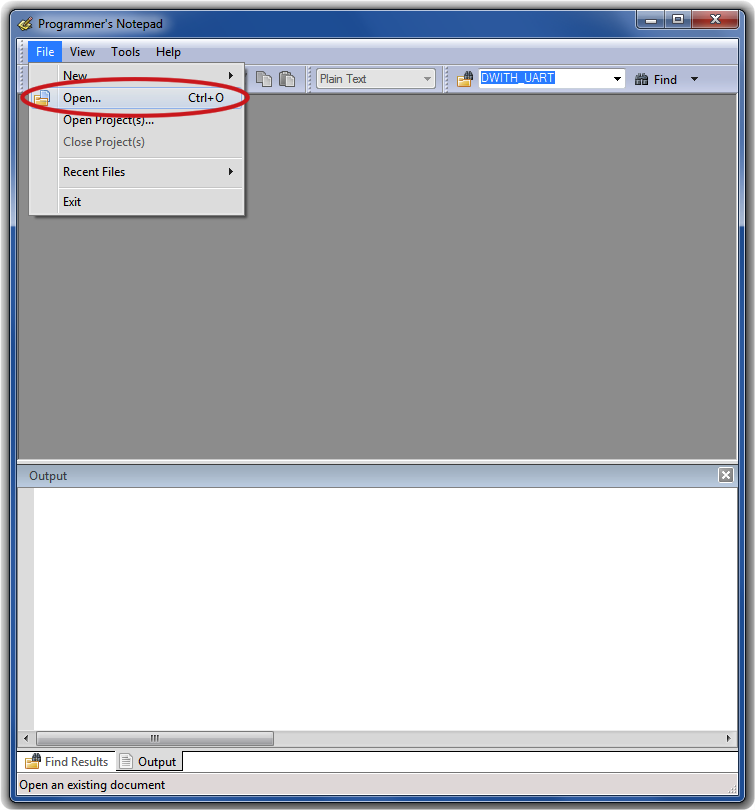
\includegraphics[width=.85\textwidth]{../PNG/Notepad_open.png}
    \caption{Otevření \lname{Makefile}}
  \end{subfigure}
  ~
  \begin{subfigure}[b]{.5\textwidth}
    \centering
    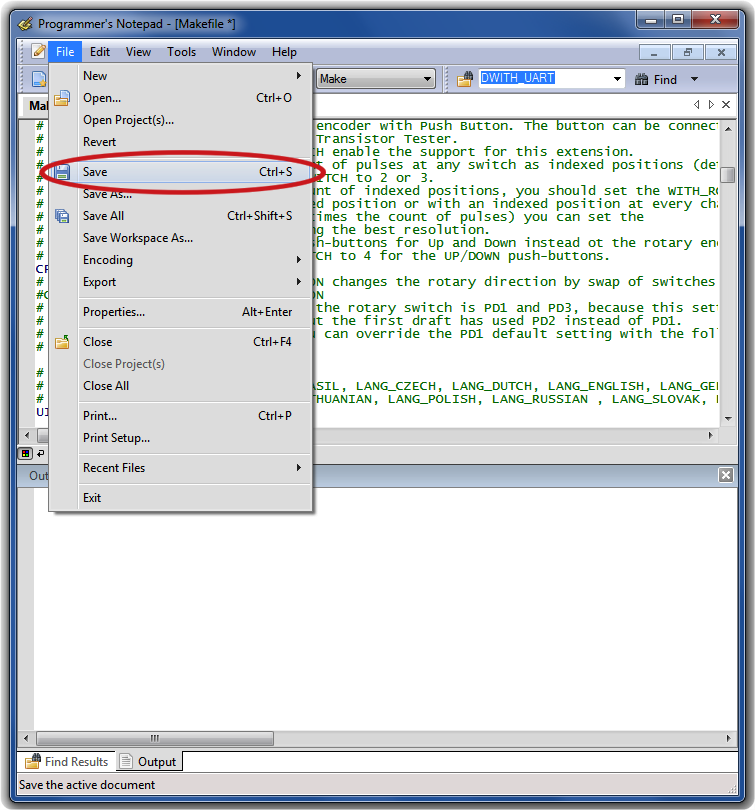
\includegraphics[width=.85\textwidth]{../PNG/Notepad_save.png}
    \caption{Uložení \lname{Makefile}}
  \end{subfigure}
  \caption{Použití programu WinAVR}
  \label{fig:WinAVR1}
\end{figure}

Následující obrázky \ref{fig:WinAVR2} zobrazují nabídku menu Nástroje programu Poznámkový blok
programu přeložení programu (Make All) a k naprogramování ATmega pomocí 'avrdudu'.

\begin{figure}[H]
  \begin{subfigure}[b]{.5\textwidth}
    \centering
    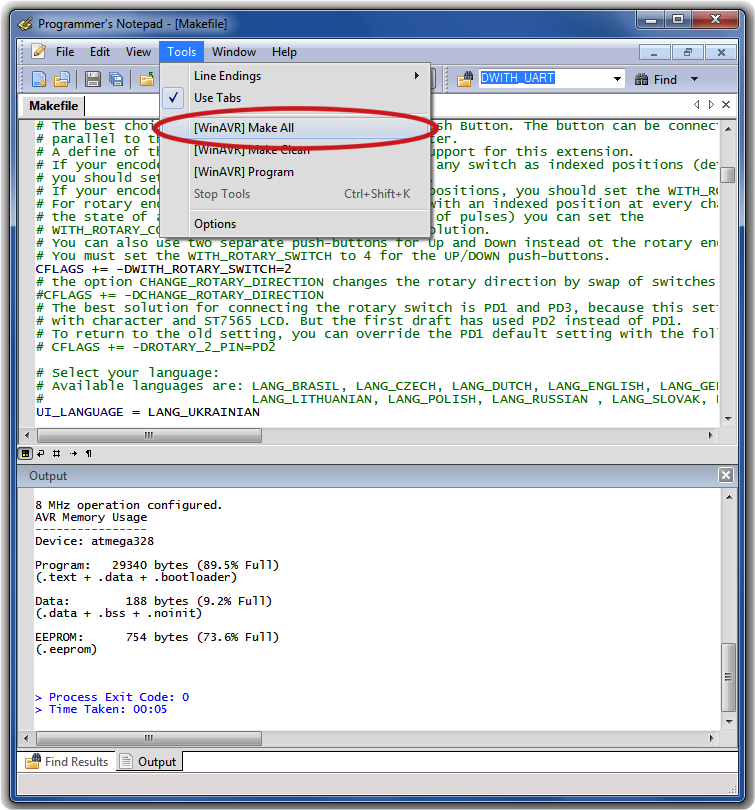
\includegraphics[width=.85\textwidth]{../PNG/Notepad_make.png}
    \caption{Vytvořit data programu (.hex/.eep)}
  \end{subfigure}
  ~
  \begin{subfigure}[b]{.5\textwidth}
    \centering
    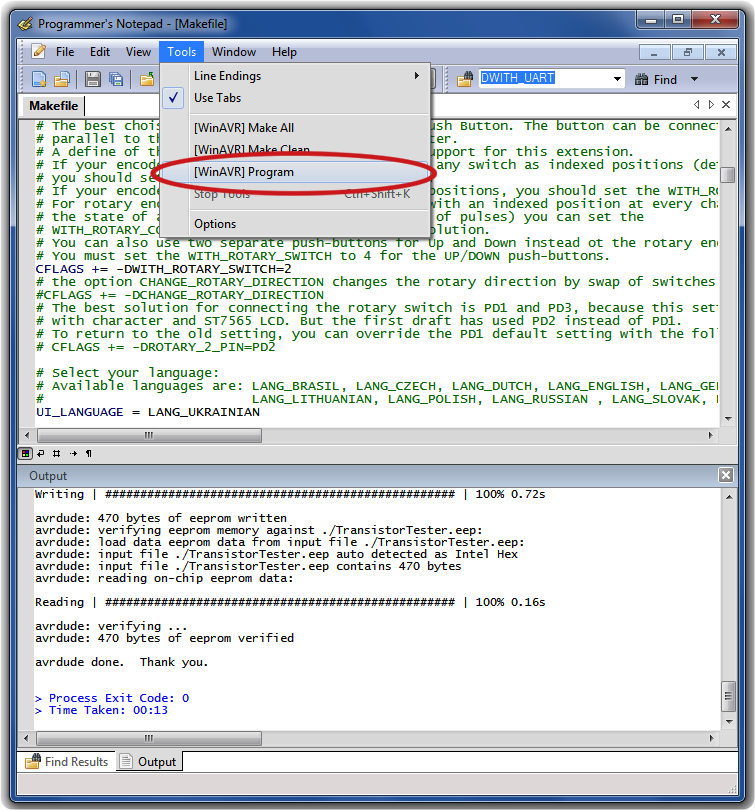
\includegraphics[width=.85\textwidth]{../PNG/Notepad_program.png}
    \caption{Naprogramovat ATmega}
  \end{subfigure}
  \caption{Obsluha WinAVR s Notepadem}
  \label{fig:WinAVR2}
\end{figure}

\section{Hledání chyb}
U většiny problémů vám na obrazovce LCD chybí text.
Nejprve byste měli zkontrolovat, zda slabě svítí LED dioda na desce, když stisknuté tlačítko start
uvolníte.

\begin{description} \setlength{\itemsep}{0em}

\item[Zařízení se nezapne]  
Pokud stisknete tlačítko Start a kontrolka se nerozsvítí, ale napětí VCC má správnou hodnotu,
nezapne se mikrokontrolér správně.
Mikrokontrolér má jako první úlohu, přepnout výstup PD6 na \(5V\).
Pokud držíte tlačítko start stisknuté, je napájení tak jako-tak zapnuté.
V tomto stavu je možné zkontrolovat hodnotu VCC napětí a navíc hodnotu napětí na výstupu PD6.
Má-li VCC-napětí správnou hodnotu (\(5V\)) ale napětí na výstupu PD6 leží pod \(4V\) není
mikrokontrolér správně zapnutý.
V takovém případě byste měli zkontrolovat, zda jsou data programu pro paměť flash nahrány
pro správný typ procesoru a zda má procesor správně nakonfigurované (fuses).
Když ATmega výstup PD6 přepne na \(5V\) ale provozní napětí po puštění tlačítka start vypne,
je obtížnější tu příčinu nalézt Nejprve můžete LED zkratovat a zkusit to znovu.
Pokud se testovací zařízení spustí, je možná LED dioda zapojena obráceně.
Pokud to není příčinou, mohl by být důvodem nedostatečný zesilovací proud tranzistoru T3 (BC557C).
Proud do báze T3 je nižší, když mikrokontrolér zapne LED než když tlačítko "stisknuté".

\item[Na LCD displeji nelze číst] 
Zkontrolujte napětí na kontrastním pinu (pin 3) LCD displeje.
Pomocí trimru nastavte hodnotu na hodnotu zadanou v datovém listu a optimalizujte ji
vizuální prohlídkou.
Pokud máte displej s vysokou teplotou, potřebujete pro provoz záporné kontrastní napětí.
V tomto případě lze ke generování záporného napětí z pozitivních \(5V\), použít integrovaný obvod ICL ~ 7660.
Tester může být použit a nakonfigurován pro mnoho různých řadičů s různými typy připojení.
Nezapomeňte zkontrolovat, zda se software shoduje s vaším displejem.
Pokud LCD displej nic neukazuje a pokud je podsvícení zapnuté
měli byste odpojit napájení a zkontrolujte všechna čtyři datová připojení i oba řídicí signály.
Pokud jsou všechny tyto spojovací vodiče v pořádku, vidím jako příčinu pouze možnost nesprávné
časové posloupnosti řídicích signálů.
Důvodem pro to může být, že řídicí jednotka displeje LCD je pomalejší než je software ATmega očekává.
Mohlo by se také stát, že ATmega je v chodu na nesprávné frekvenci.
Zkontrolujte pro jakou taktovací frekvenci je software přeložena a zda jsou ATmega fuse pro
tuto rychlost správně nastaveny.
Nastavenou frekvenci najdete v příslušném \lname{Makefile}.
Pokud je tester vyroben bez vypínací automatiky, můžete zapojit zkušební LED diody přímo na
zkoušené piny, abyste zjistili, zda program funguje.
Pokud LED bliká, program běží. V tomto případě musí být chyba v připojení LCD displeje.
 U některých grafických displejů může být kontrast nastaven pomocí funkce menu.
Pokud jste náhodně nastavili špatný kontrast, tak také není displej čitelný a tester není možné
ovládat.
Zde se můžete jen pokusit zjistit, zda je z boku (šikmé) něco vidět a obnovit kontrast pomocí
nabídky menu. Pokud to nefunguje, můžete přepsat program EEprom ATmega s programátorem ISP a obnovit jeho hodnotu.

\item[Něco, ale ne vše, je na LCD displeji čitelné] 
Zkontrolujte, zda byla data EEPROM vložena do Eepromu ATmega.
Po správném zavedení všech dat programu byste měli zkontrolovat nastavení frekvence v (\lname{Makefile})
a nastavení ATmega (fuses).

\item[Měření je příliš pomalé a kapacity jsou měřeny faktorem 8 příliš malým.] 
Používáte software přeloženou pro \(8MHz\) s frekvencí \(1MHz\).
Nakonfigurujte u ATmega (fuses) správně.

\item[Měření dává podivné výsledky.]  
Zkontrolujte, zda je stále připojen programovací konektor ISP. Konektor ISP by během měření neměl být zapojen.
Velmi často je důvodem pro nesprávné výsledky měření, že software používá volbu
AUTOSCALE\_ADC a že byla přeložena volba NO\_REF\_CAP ale kondenzátor na pinu AREF-Pin má stále
hodnotu \(100nF\).
Příčinou může být také použití nesprávných součástek,
nesprávná montáž nebo reziduální zbytky pájky a tavidla FluX mohou ovlivňovat měření.
Zkontrolujte prosím, pokud je to možné, funkcí automatického testu kalibrace její nastavení.
Podrobnosti naleznete v kapitole \ref{sec:selftest}.
Jinak zkontrolujte vizuálně desku a zkontrolujte hodnoty odporů s ohmmetrem.
Pro tento test můžete použít ATmega piny,
Můžete například měřit odpor R1 mezi pinem 23 a pinem 14.
Podívejte se do schématu \ref{fig:ttester} pro podrobnosti.
Nemusíte odstraňovat mikrokontrolér, ale zdroj napájení by měl být odpojen.

\item[Tester se vypne po 2 sekundách.]  
V tomto případě schází pull-up odpor u vstupu PD7, nebo je tlačítko trvale stisknuto.
Software vypíná interní pull-up odpory pro ovlivňování výsledků měření.\\ Proto je vyžadován externí odpor.

\item[Tester ukazuje stále jen Vext=xx.xV ve druhém řádku.]
Také zde chybí pull-up odpor u vstupu PD7, nebo je tlačítko trvale stisknuto.
Kromě toho je software je také bez sériového výstupu (bez volby WITH\_UART) a bez vnitřních
pull-Up odporů (s volbou PULLUP\_DISABLE) konfigurovaná.\\
Přidejte pull-Up odpor na PD7.

\end{description}
